\section[KUV mit minimalem Residuum]{Krylov-Unterraum-Verfahren mit minimalem Residuum}

{\bf Gegeben: }
\begin{quote}
$A \in \cnn$ mit $A \neq A^H$,  $A$ regul\"ar.
\end{quote}
{\bf Ziel: }
\begin{quote}
L\"ose $Ax = b$ mit Startvektor $x^0$ und $r^0 = b-Ax^0$.
\end{quote}
{\bf Idee:}
\begin{quote}
Bestimme ONB von $K_m(A,r^0)$ mit Arnoldi-Prozess und errechne $x^m \in x^0 + K_m(A,r^0)$, so dass
\end{quote}
\[
\|b-Ax^m\|_2 = \underset{x \in x^0 + K_m(A,r^0)}{\min} \|b-Ax\|_2.
\]

{\bf Ansatz:}
\begin{quote}
$x = x^0 + V_m z^m$ mit $z^m = \left(z_1,\cdots,z_m\right)^T \in \co^m$ sowie
$V_m = \left[ v^1,\cdots,v^m \right]$.
\end{quote}

Damit erhalten wir
\[
b - Ax = r^0 - AV_m z^m = r^0 - V_{m+1}H_{m+1,m}z^m.
\]

Mit $r^0 = h_{1,0} v^1$ und $h_{1,0} = \|r^0\|$ gilt nun
\[
b-Ax = V_{m+1} \left[
\left(%
\begin{array}{c}
  h_{1,0} \\
  0 \\
  \vdots \\
  0 \\
\end{array}%
\right) - H_{m+1,m} z^m \right]
\]
und somit
\[
\|b-Ax\|_2 = \|h_{1,0}e^1 - H_{m+1,m}z^m\|_2.
\]
Hierbei ist $e^1$ der erste Einheitsvektor in $\co^{m+1}$,
$H_{m+1,m} \in \mathbb{C}^{(m+1)\times m}$
aber $z \in \mathbb{C}^m$.

\clearpage

{\bf Exkurs:}

\begin{quote}
Zu l\"osen ist also ein "uberbestimmtes Least Squares Problem $Bx = c$ mit
$B\in \mathbb{C}^{k \times l}, \; k > l$. Gesucht ist
ein $x$, welches $\| Bx-c \|_2^2$ minimiert. Dies findet man unter Verwendung der
QR-Faktorisierung.

{\bf Ansatz:}
\begin{quote}
Faktorisiere $ B = QR$ mittels QR-Zerlegung. Dann folgt
\end{quote}
\begin{align*}
\|Bx-c\|_2^2 &= \|Q^H(Bx-c)\|_2^2\\
&= \|Rx - Q^Hc\|_2^2.
\end{align*}
Das Minimum wird erreicht f\"ur
\[
x = R_1^{-1}( (Q^Hc)(1:l) ),
\]
wobei
\[
R = \left(\begin{array}{ccc} & R_1 & \\
    0 & \cdots & 0 \end{array}
    \right), \enspace R_1 \in \co^{l\times l} \mbox{ obere Dreiecksmatrix }.
\]
\end{quote}

In unserem Falle ist $H_{m+1,m}$ eine obere Hessenberg Matrix. Ihre QR-Fak\-to\-ri\-sierung
kann mittels Jacobi Rotationen bestimmt werden. Es kann sogar $Q$ in der
QR-Faktorisierung von $H_{m+1,m}$ auf die f"ur $H_{m+2,m+1}$ aufdatiert werden.

\bigskip

{\bf Notation:}
\[
Q_{m+1} H_{m+1,m} = R_{m+1,m} \enspace \mbox{QR-Faktorisierung}
\]
mit
\[
Q_{m+1} = J_m^{(m+1)}\cdots J_1^{(m+1)},
\]
wobei $J_j^{(m+1)}$ eine Jacobi Rotation in $\co^{m+1}$ auf den Zeilen $j$
und $j+1$ ist, welche das `untere Nebendiagonalelement' $h_{j+1,j}$ eliminiert,
\[
J_j^{(m+1)} = \left(%
\begin{array}{cccc}
  I &  &  &  \\
   & \bar{c}_j & \bar{s}_j &  \\
   & -s_j & c_j &  \\
   &  &  & I \\
\end{array}%
\right).
\]
Um anzugeben, wie man $J_m^{(m+1)}$ bestimmt, beobachten wir zun\"achst
\begin{eqnarray*}
J_{m-1}^{(m+1)} \cdots J_1^{(m+1)} H_{m+1,m} &=& J_{m-1}^{(m+1)} \cdots J_1^{(m+1)}
    \left(\begin{array}{c|c} 
  H_{m,m-1}& \begin{array}{c}
           h_{1,m} \\
  \vdots \\
h_{m,m}
  \end{array}\\
\hline
  0         & h_{m+1,m}
  \end{array}
 \right) \\
&=&
    \left( \begin{array}{cc}
  R_{m,m-1} & \eta^{(m)} \\
  0         & h_{m+1,m}
  \end{array}
 \right)
\end{eqnarray*}
mit
\[
\eta^{(m)} = (r_{1,m},\ldots,r_{m-1,m},\eta_{m,m})^T,
\]
wobei
\begin{eqnarray*}
r_{1,m} &=& \bar{c}_1h_{1,m} + \bar{s}_1h_{2,m}, \\
\eta_{1,m} &=& -s_1h_{1,m} + c_1h_{2,m}, \\
r_{2,m} &=& \bar{c}_2\eta_{2,m} + \bar{s}_2h_{3,m}, \\
\eta_{2,m} &=& -s_2\eta_{1,m} + c_2h_{3,m}, \\
& \vdots & \\
\eta_{m,m} &=& -s_{m-1}\eta_{m-1,m} + c_{m-1}h_{m,m} .
\end{eqnarray*}
Damit erhalten wir f"ur die Parameter $c_m,s_m$ der Jacobi Rotation
$J^{(m+1)}_m$, welche $(0,\ldots,0,\eta_{m,m},h_{m+1,m})^T$ abbildet auf
$(0,\ldots,0,r_{m,m},0)^T$ die Werte 
\begin{equation} \label{rotparam_eq}
  c_m = \eta_{m,m}/\sqrt{|\eta_{m,m}|^2 + |h_{m+1,m}|^2}, \
s_m = h_{m+1,m}/\sqrt{|\eta_{m,m}|^2 + |h_{m+1,m}|^2}  \hspace*{-0.6cm}
\end{equation}
und
\[
r_{m,m} = \bar{c}_m\eta_{m,m} + \bar{s}_mh_{m+1,m} = \sqrt{|\eta_{m,m}|^2 + |h_{m+1,m}|^2} .
\]

% Vorlesung vom 20.05.03

Die L"osung des LS-Problems
\[\min \|h_{1,0} e^1 - H_{m+1,m} z^m \|_2 \]
lautet damit
$$ z^m = h_{1,0} R_m^{-1} ((Q_{m+1} e^1)(1:m)), \enspace \mbox{ wobei }
 R_{m+1,m} = \left( \begin{array}{c} R_m \\
                    0 \cdots 0
                    \end{array}
             \right),
$$
und der Wert des Minimums ist
$$ h_{1,0} ( Q_{m+1} e^1)_{m+1}. $$
Dieser Wert kann ohne Kenntnis von $z^m$ wie folgt bestimmt werden:
Setze 
$$ Q_m e^1=h_{1,0} \left(\begin{array}{c}
                        \epsilon_1\\
                        \vdots\\
                        \epsilon_{m-1} \\
                        \tilde{\epsilon}_{m}
               \end{array}\right). $$
Dann ist
\[
Q_{m+1}e^1 = J_m^{(m+1)} \left( \begin{array}{cc} Q_m & 0 \\
                                               0 & 1 
                                  \end{array}
                         \right) e^1
 = J_m^{(m+1)} \cdot
      \left(\begin{array}{c}
                        \epsilon_1\\
                        \vdots\\
                        \epsilon_{m-1} \\
                        \tilde{\epsilon}_{m} \\
                          0
               \end{array}\right)
 =
\left(\begin{array}{c}
                        \epsilon_1\\
                        \vdots\\
                        \epsilon_{m} \\
                        \tilde{\epsilon}_{m+1}
               \end{array}\right),
\]
mit
\begin{align*}
  \epsilon_m & =  \tilde{\epsilon}_m\overline{c}_m, \\
  \tilde{\epsilon}_{m+1} & =  \tilde{\epsilon}_m\overline{s}_m. \\
\end{align*}
Insbesondere gilt
$$ \tilde{\epsilon}_{m+1} = \prod \limits_{j=1}^{m} \overline{s}_j ,$$
so dass wir f"ur den Wert des Minimums den Ausdruck
\[
  h_{1,0}\tilde{\epsilon}_{m+1} = \|r^0\| \cdot \tilde{\epsilon}_{m+1}
\]
erhalten.

Wir haben jetzt alle Zutaten f"ur das Verfahren
GMRES (Generalized Minimal Residual):

\clearpage


\begin{alg}[GMRES (Saad, Schultz, 1986)] \label{GMRES_alg}
~               % um "3.3 Algorithmus" aus dem Kasten rauszubekommen
\vspace*{-2\baselineskip}       % um den Leeraum zu entfernen
\begin{algorithm}
  \begin{algorithmic}
    \STATE w\"ahle $x^0$, setze $r^0 = b-Ax^0,\ \rho_0=h_{1,0}=\|r^0\|_2 $
    \FOR{$m = 1,2, \dots$, bis $\rho_m$ klein genug}
      \STATE bestimme n\"achsten Vektor $v^m$ und Koeffizienten
    $h_1^m, \ldots ,h_{m+1}^m$ aus Arnoldi-Prozess
      \STATE bestimme $s_m,c_m$ nach \eqnref{rotparam_eq}
      \STATE datiere $\epsilon_m$ und $\tilde{\epsilon}_{m+1}$ auf
      \STATE setze $\rho^m = \rho_{m-1}\cdot \overline{s}_m $
             \enspace \COMMENT{ $\rho_m = \|r^m\|$} 
      \IF{$\rho_m$ klein genug}
          \STATE l\"ose $R_{m} z^{m} =  \left( \epsilon_1, \ldots, \epsilon_m \right)^T$
          \STATE setze $x^{m} = x^0 + V_{m} z^{m}$
      \ENDIF
    \ENDFOR
  \end{algorithmic}
\end{algorithm}
\end{alg}

\begin{bem}
 Speicher- und Rechenaufwand (ohne MVMs) verh\"alt sich wie $\mathcal{O}(mn + m^2)$
 $\curvearrowright$ Verfahren wird schnell impraktikabel.
\end{bem}
Es bezeichne $x^m$ die GMRES-Iterierte nach jedem Schritt, also die L\"osung
von $$\min\limits_{x \in x^0+K_m(A,r^0)} \|b-Ax\|_2. $$
Dann gilt nat"urlich $$ \|r^0\|\geq\|r^1\|\geq \ldots .$$
Das folgende Beispiel zeigt, dass hier lange Gleichheit herrschen kann.

\begin{bsp} \label{stagnation_bsp}
Sei
\[
 A = \left(\begin{array}{cccc}
                        0 &        & & 1\\
                        1 & \ddots & & 0\\
                          & \ddots & \ddots & \vdots \\
                          & & 1 & 0
               \end{array}\right),\enspace x^0=0,\;  b=e^1=r^0.
\]
Dann ist $K_m(A,r^0)=  \spann\{e^1,\ldots,e^m\}$, $e^i$ = $i$-ter Einheitsvektor.
L\"osung von  
$$\min\limits_{x \in K_m(A,r^0)} \|e^1-Ax\|_2, $$
ist f"ur $m=1,2,\ldots,n-1$ wegen
$Ax\in  \spann\{e^2,\ldots,e^{m+1}\}$ stets $x^m=0$.
Es gilt also f\"ur die GMRES-Iterierten
$$ x^0=x^1=\ldots=x^{n-1}=0,\; x^n=e^n = A^{-1}b $$ und 
$$ r^0=r^1=\ldots=r^{n-1}=e^1, $$
also
$$\|r^0\|=\ldots=\|r^{n-1}\|=1. $$
Beachte: $\spek(A)=\{ e^{\frac{2\pi ik}{n}} , \;  k=0,\ldots,n-1\} $. Ein so
um die 0 verteiltes Spektrum ist f"ur KUV prinzipiell schwierig, weil die
Verfahrenspolynome ja $p(0) = 1$ erf"ullen m"ussen.
\end{bsp}

Idee f\"ur "`praktikable"' GMRES-Variante: "`Restarted"'GMRES=GMRES($k$)
mit restart Wert $k$.
\begin{alg}[GMRES($k$)]
~               % um "3.3 Algorithmus" aus dem Kasten rauszubekommen
\vspace*{-2\baselineskip}       % um den Leeraum zu entfernen
\begin{algorithm}
  \begin{algorithmic}
    \STATE w\"ahle $x^0$
    \FOR{$m = 1,2,\dots$}
      \STATE f\"uhre $k$ Schritte von GMRES aus mit Startvektor $x^{m-1}$
      \STATE Ergebnis ist $x^m$
    \ENDFOR
  \end{algorithmic}
\end{algorithm}
\end{alg}
Es ist nun $$ x^m \in x^{m-1}+K_k(A,r^{m-1}), r^{m-1}=b-Ax^{m-1},$$
aber es gilt i.A. {\em nicht}
\[
x^m \in x^0 + K_{km}(A,r^0).
\]

\begin{bem}
Berechnung von $x^m$ aus $x^{m-1}$ kostet $k$ MVM. Speicheraufwand
ist $n\cdot k+\mathcal{O}(n+k^2)$, entsprechend f\"ur Rechenaufwand.
\end{bem}

Auch bei restarted GMRES gilt  $\|r^0\| \geq \|r^1\|\geq \ldots $.
Jetzt besteht allerdings die Gefahr der \emph{Stagnation}, d.h. 
$\lim\limits_{m\rightarrow\infty} \|r^m\|\not=0.$
\begin{bsp}
Seien $A,x^0,b$ wie in Beispiel \ref{stagnation_bsp}.
F\"ur alle $k<n$ stagniert GMRES($k$) mit $x^m=0$ f\"ur alle $m$.
\end{bsp}

{\bf Exkurs:} Ein Modellproblem (Modellproblem III) mit
unsymmetrischer Matrix.
\begin{equation} \label{conv_diff_eq}
\left\{ \quad
\begin{array}{rcl}
\Delta u + \epsilon u_x &=& f  \text{ f\"ur } (x,y)\in\Omega=(0,1)\times(0,1)\\
u &=& g   \text{ f\"ur } (x,y)\in \partial \Omega 
\end{array}
\quad
\right.
\end{equation}
Man nennt dies eine Konvektions-Diffusions-Gleichung mit Konvektionsterm
$\epsilon u_x$.
Ansatz mit Diskretisierung auf Gitterpunkten $(ih,jh),\ i,j=1,\ldots,N,$ $h=\frac{1}{N+1}$,
ergibt einen 5-Punkte-Stern:
\begin{eqnarray*}
\Delta u(ih,jh) & \approx & \frac{4u_{i,j}-u_{i-1,j}-u_{i,j-1}-u_{i+1,j}-u_{i,j+1}}{h^2}, \\
 u_x(ih,jh) & \approx & \frac{u_{i+1,j}-u_{i-1,j}}{2h}.
\end{eqnarray*}

\begin{figure}
\setlength{\unitlength}{0.02cm}
\begin{center}
 \begin{picture}(250,200)
   \multiput(0,0)(50,0){6}{%
    \multiput(0,0)(0,50){5}{
      \circle*{5}
    }
  }
\footnotesize
 \put(107,110){$+4$}
 \put(15,110){$-1-\epsilon\frac{h}{2}$}
 \put(150,110){$-1+\epsilon\frac{h}{2}$}
 \put(107,60){$-1$}
 \put(107,160){$-1$}
\normalsize
 \drawline(54,100)(154,100)
 \drawline(104,50)(104,150)
 \end{picture}
\end{center}
\caption{5-Punkte-Stern f"ur die Konvektions-Diffusionsgleichung \eqnref{conv_diff_eq}}
\end{figure}

Wie fr\"uher nehmen wir $f=0$ und 
\begin{eqnarray*}
g_{0,j} &=& jh \\
g_{N+1,j} &=& 1-jh \\
g_{i,0} &=& ih \\
g_{i,N+1} &=& 1-ih.
\end{eqnarray*}
Die zugeh\"orige Matrix ist unsymmetrisch.

\begin{aufg} \label{GMRES_auf}
F\"ur $\epsilon=1,50$ und $N=10,20,40$ berechne man mit MATLAB Folgendes:
\begin{enumerate}
 \item Das vollst\"andige Spektrum der Matrix (Plot!) und
 \item die Konvergenzgeschichte von GMRES($k$) f\"ur verschiedene Werte von
  $k=1,2,4,8,16,32,64$.
\end{enumerate}
\end{aufg}

\begin{figure}
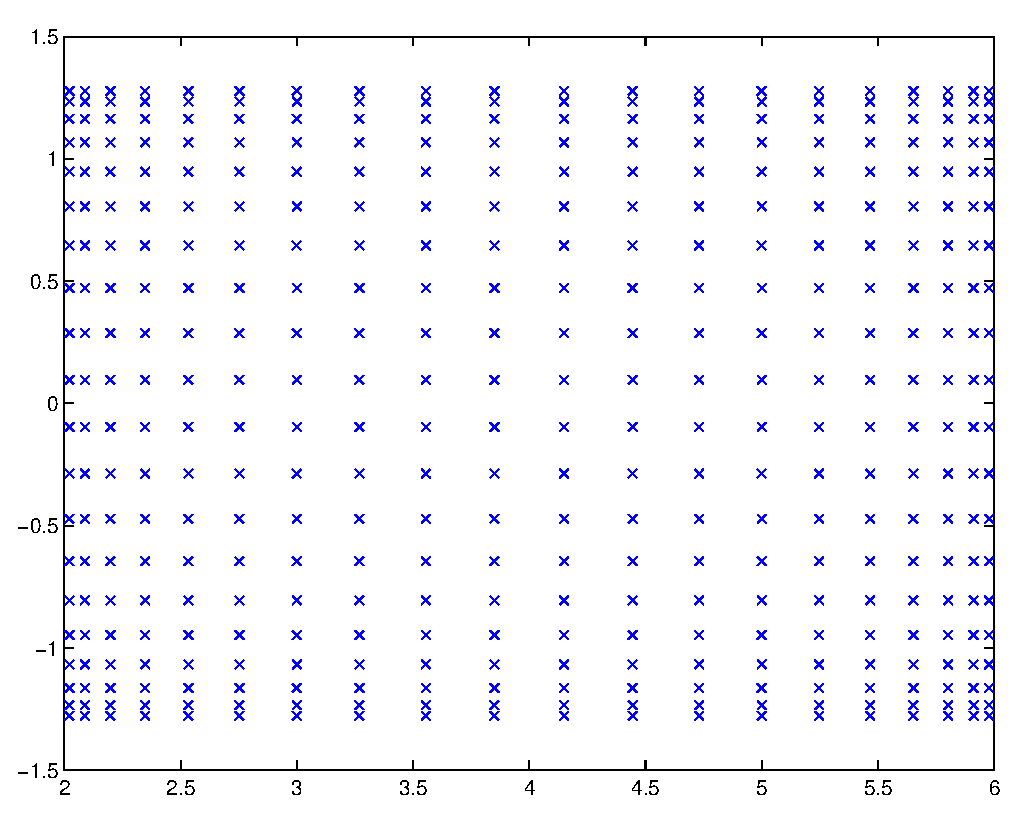
\includegraphics[scale=0.35]{eps/speke50n20.eps}
\hfill
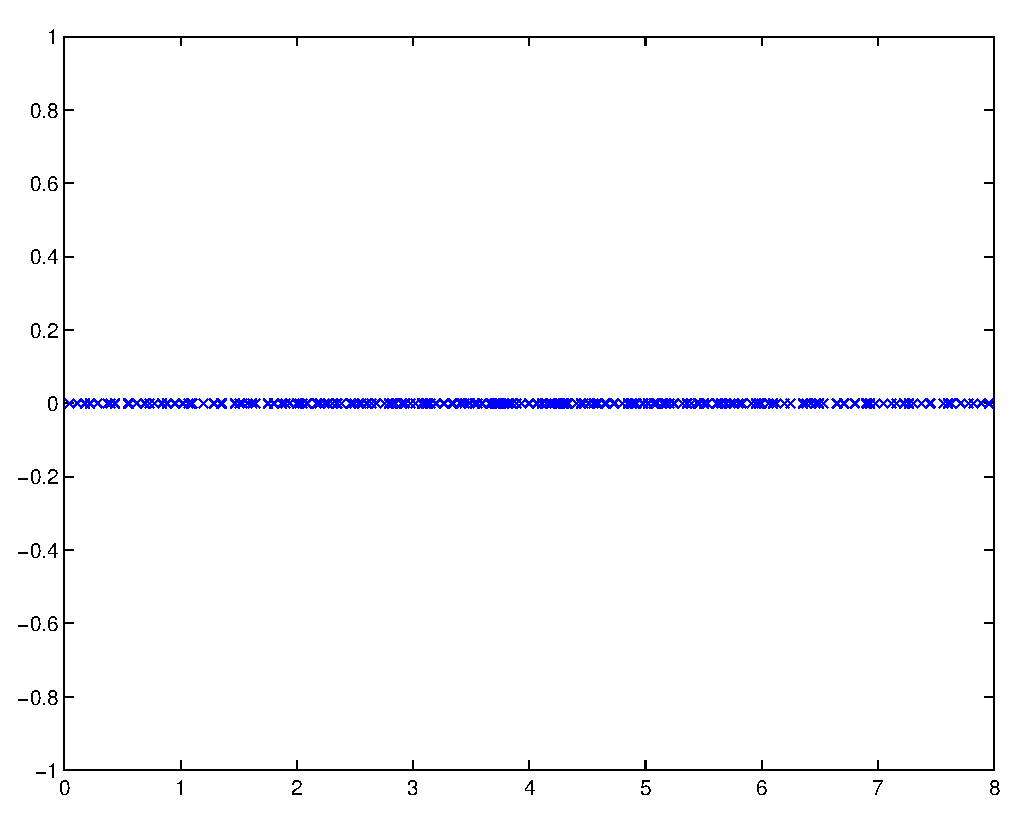
\includegraphics[scale=0.35]{eps/speke1n20.eps}
\caption{Spektrum von $A_{\epsilon}$ f"ur $N=20$ und $\epsilon = 50$ (links)
und $\epsilon = 1$ (rechts)}
\end{figure}

\begin{figure}
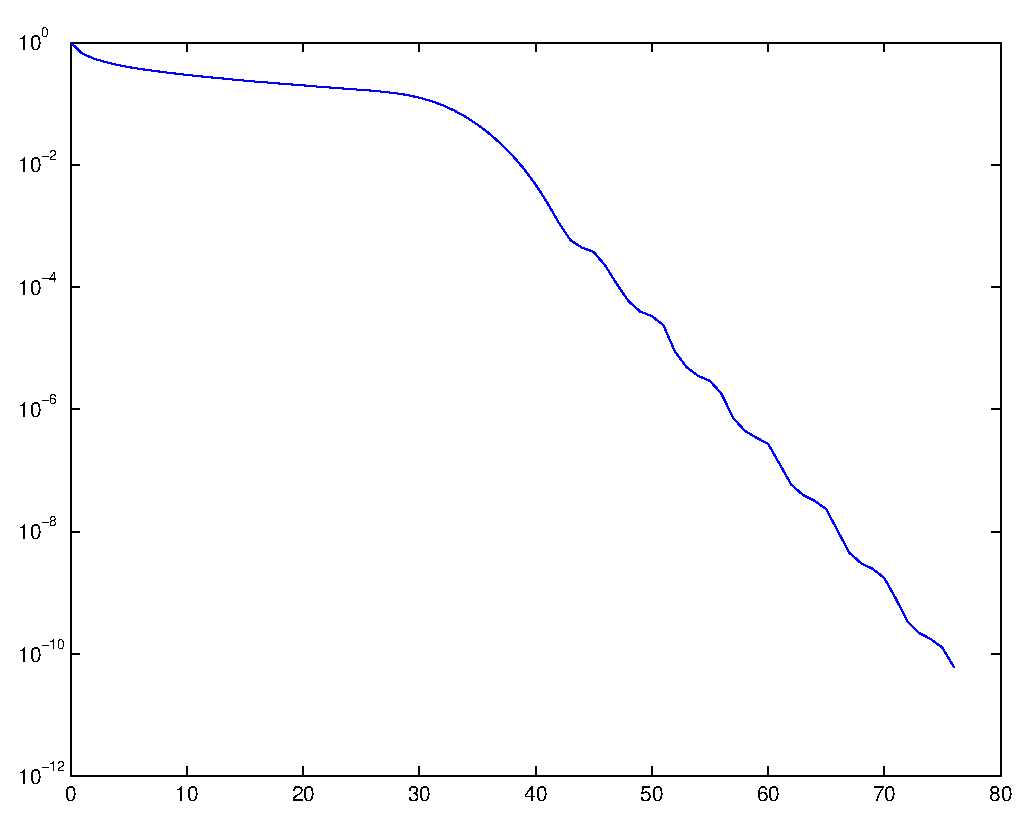
\includegraphics[scale=0.35]{eps/mp3e50n20k1.eps}
\hfill
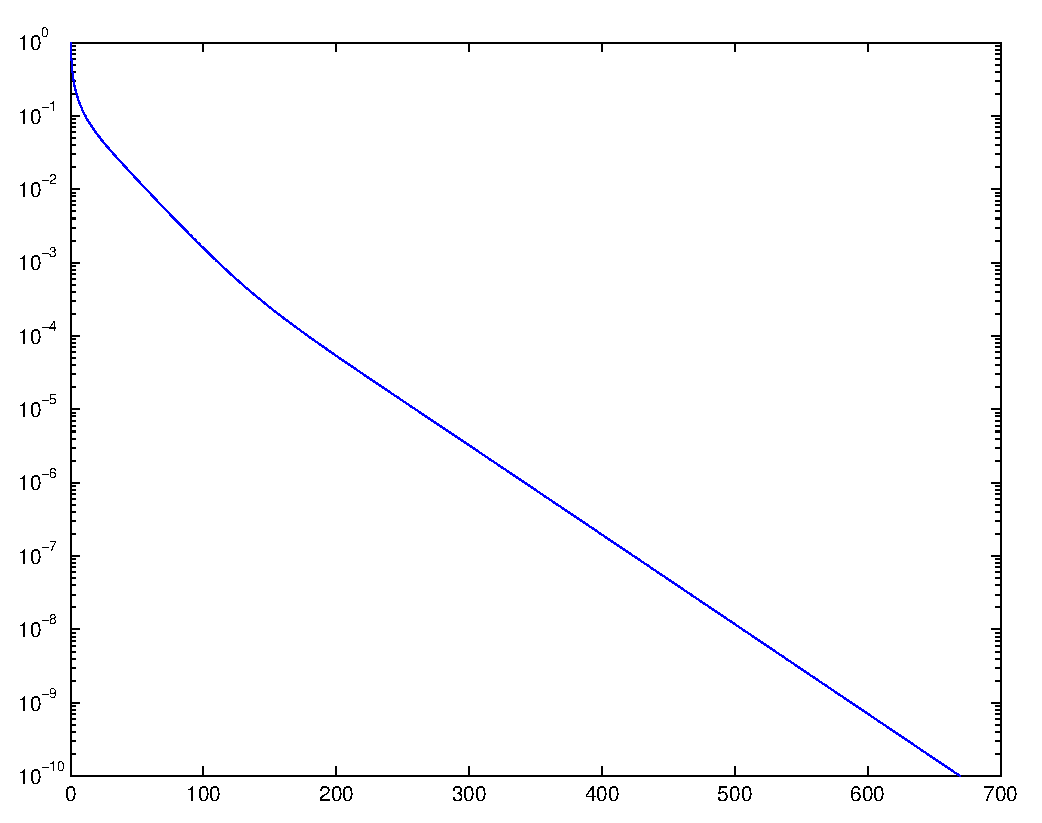
\includegraphics[scale=0.35]{eps/mp3e1n20k1.eps}
\\
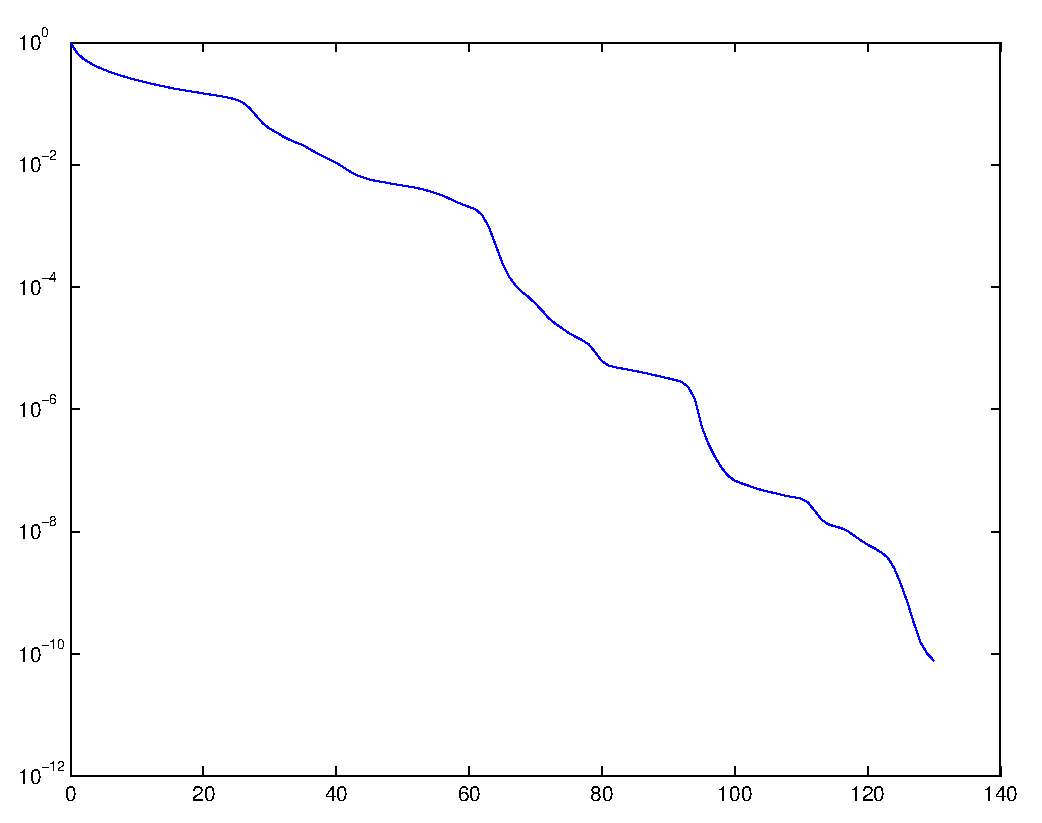
\includegraphics[scale=0.35]{eps/mp3e50n20k16.eps}
\hfill
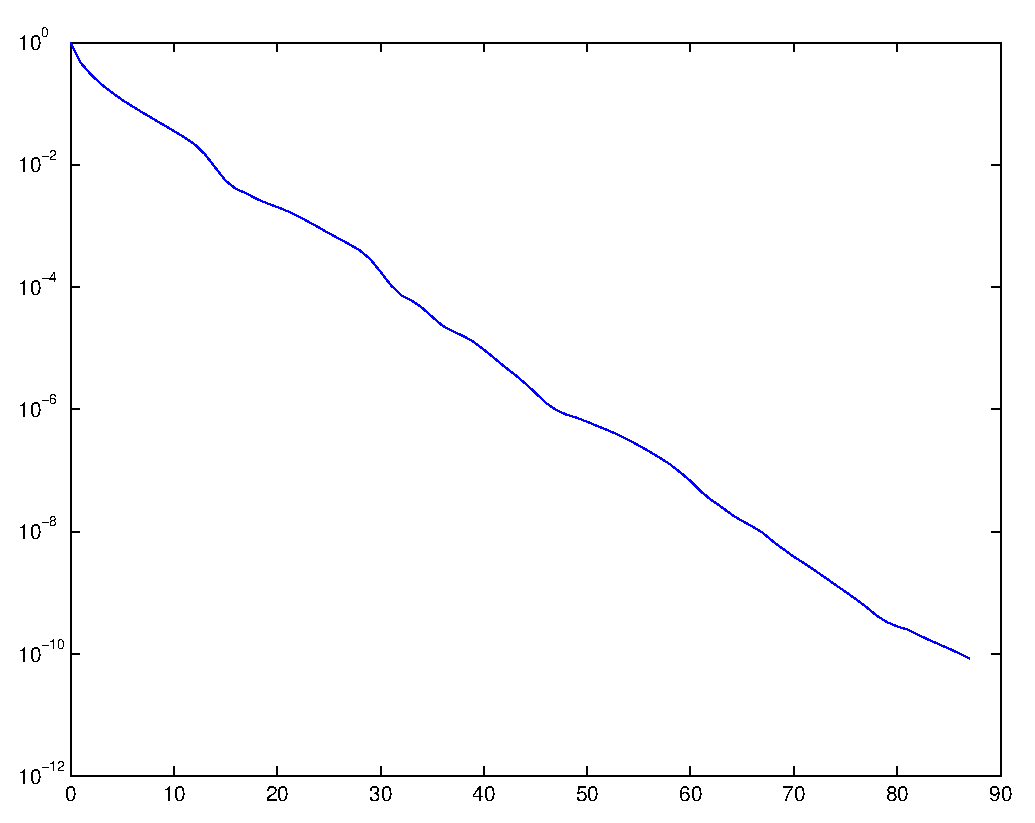
\includegraphics[scale=0.35]{eps/mp3e1n20k16.eps}
\\
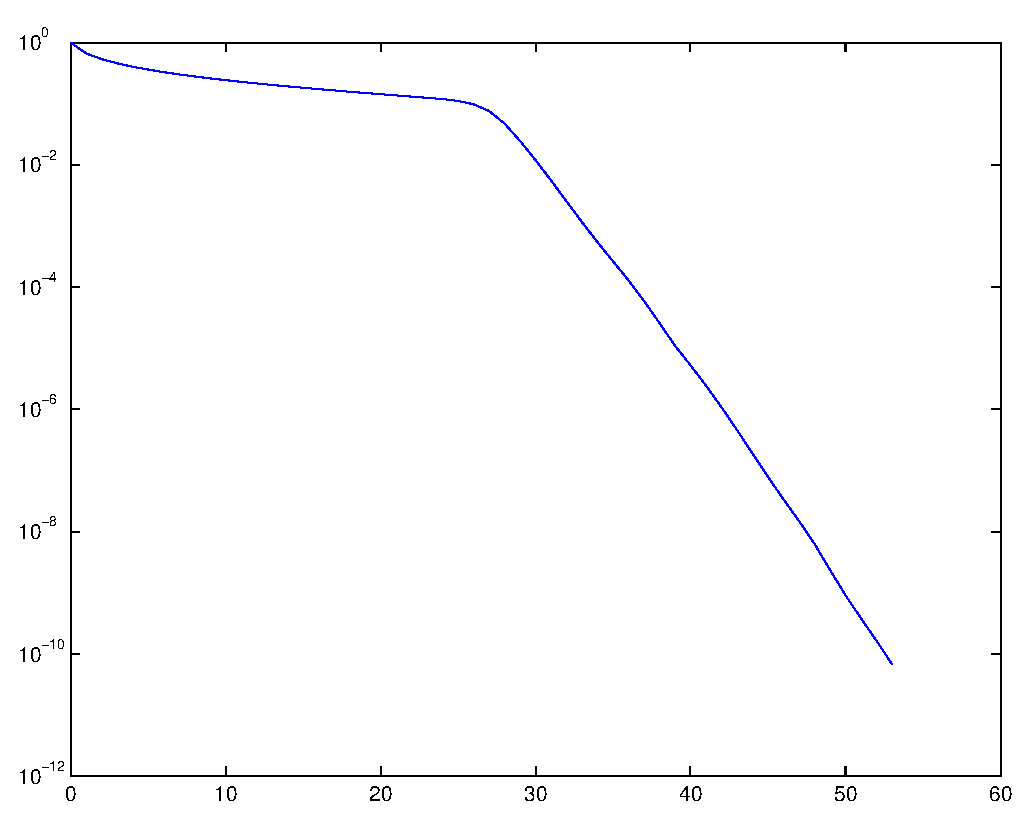
\includegraphics[scale=0.35]{eps/mp3e50n20k64.eps}
\hfill
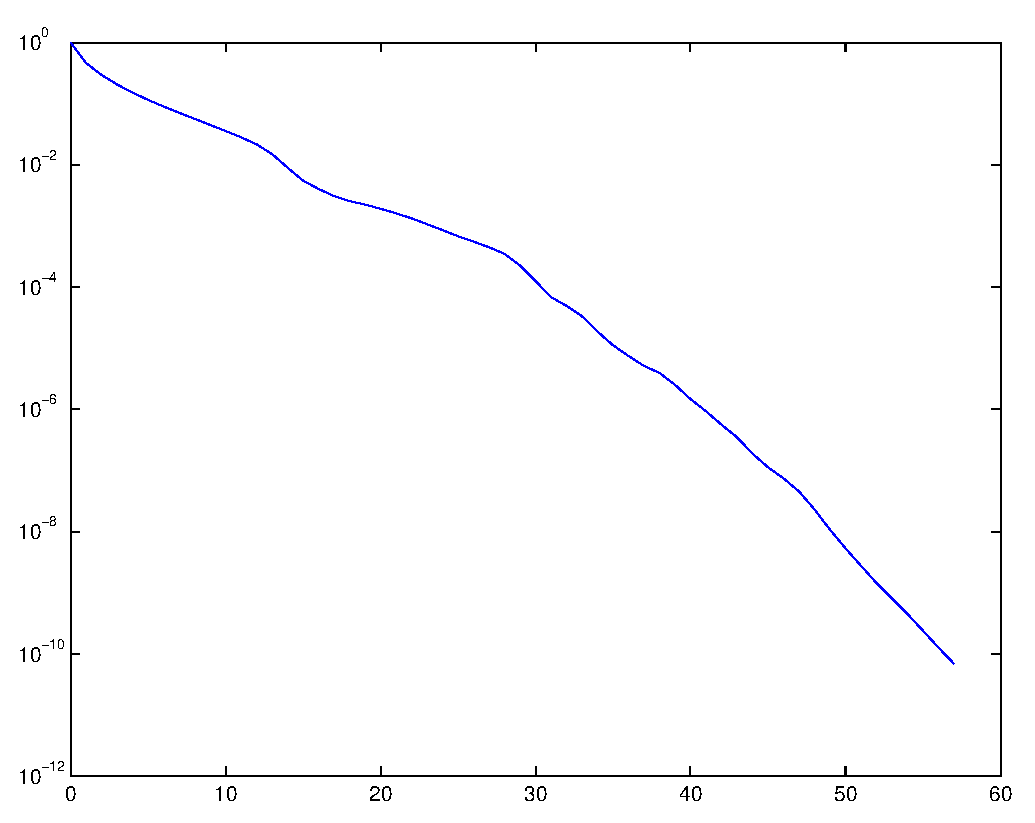
\includegraphics[scale=0.35]{eps/mp3e1n20k64.eps}
\caption{Konvergenzgeschichte (Norm des Residuums als Funktion der 
Iterationszahl) f"ur GMRES($k$), $k=1,16,64$). Linke Spalte:
$N=20, \epsilon = 50$, rechte Spalte: $N=20, \epsilon = 1$}
\end{figure}


Spezialfall f\"ur GMRES: $A=A^H$, aber nicht notwendig hpd. 
Dann: Arnoldi- wird zum Lanczos-Prozess, d.h. kurze Rekursionen werden m\"oglich.
\begin{eqnarray*}
 H_{m+1,m} \rightarrow T_{m+1,m}=
 \left(\begin{array}{cccc}
                        \alpha_1  & \beta_2  & & \\
                        \beta_2   & \alpha_2 & \ddots  & \\
                                  & \ddots   & \ddots  & \beta_m \\
                                  &          & \beta_m & \alpha_{m} \\
					    &          &         & \beta_{m+1}
               \end{array}\right). 
\end{eqnarray*}
Die Berechnung der QR-Faktorisierung von $T_{m+1,m}$ vereinfacht sich:
\begin{eqnarray*}
 J_{m-1}^{(m+1)}\cdots J_{1}^{(m+1)} \cdot T_{m+1,m} & = &
 J_{m-1}^{(m+1)}\cdots J_{1}^{(m+1)} \cdot
               \left(\begin{array}{cc}
                        & 0\\
                        & \vdots\\
				& 0 \\
                        \raisebox{12pt}[-12pt]{\large $T_{m,m-1}$} & \beta_m \\
				& \alpha_m \\
				0 \ldots 0 & \beta_{m+1}
               \end{array}\right) \\
& = & \left(\begin{array}{cc}
                        & 0\\
                        & \vdots\\
				& 0 \\
				& \tilde \gamma_m \\
\quad                        \raisebox{12pt}[-12pt]{\large $R_{m,m-1}$} \quad& \tilde \beta_m \\
				& \tilde {\tilde \alpha}_m \\
				0 \cdots 0 & \beta_{m+1}
               \end{array}\right) 
\end{eqnarray*}
mit
\begin{eqnarray*}
 \tilde \gamma_m &=& \overline{s}_{m-2} \beta_m, \\
 \tilde{\tilde{\beta}}_m &=& c_{m-2} \beta_m, \\
 \tilde \beta_m &=& \overline{c}_{m-1} \tilde {\tilde{ \beta}}_m + \overline{s}_{m-1} \alpha_m, \\
 \tilde {\tilde \alpha}_m &=& -s_{m-1} \tilde {\tilde{ \beta}}_m + c_{m-1} \alpha_m.
\end{eqnarray*}
Setze nun
\begin{eqnarray*}
  {\tilde{ \alpha}}_m &=& \sqrt{|\tilde{ \tilde \alpha}_m|^2+|\beta_{m+1}|^2}, \\
 c_m &=&  \tilde {\tilde \alpha}_m /  {\tilde{ \alpha}}_m, \\
 s_m &=& \beta_{m+1} / {\tilde {\alpha}}_m.
\end{eqnarray*}
Mit
\begin{eqnarray*}
J_m^{(m+1)} = \left(\begin{array}{ccc}
                        & & \\
                        \raisebox{12pt}[-12pt]{\large I} & \raisebox{12pt}[-12pt]{\large 0}& \\
				& \overline{c}_m & \overline{s}_m \\
\raisebox{12pt}[-12pt]{\large 0}				& -s_m & c_m
               \end{array}\right) 
\end{eqnarray*}
gilt
\begin{eqnarray*}
 J_m^{(m+1)}\cdots J_1^{(m+1)} \cdot T_{m+1,m} &=&  
\left(\begin{array}{cc}
                        & 0\\
                        & \vdots\\
				& 0 \\
				& \tilde \gamma_m \\
\quad                        \raisebox{12pt}[-12pt]{\large $R_{m,m-1}$}\quad & \tilde \beta_m \\
				&  {\tilde {\alpha}}_m \\
				0 \cdots 0 & 0
               \end{array}\right) \; = \; R_{m+1,m}.
\end{eqnarray*}
$R_{m,m+1}$ hat nur drei besetzte Diagonalen.
Die GMRES-Iterierte $x^m$ erf\"ullt
$$ x^m = x^0 + V_m z^m \text{ mit } R_m z^m=\beta_1 (\epsilon_1,\ldots,\epsilon_m)^T .$$
Frage: Wie datiert man $x^m$ aus $x^{m-1}$ auf, wenn m"oglich mit kurzer Rekursion?

Es ist\begin{align*}
x^m&=x^0+V_mz^m\text{ mit }R_mz^m =\beta_1(\epsilon_1,\ldots,\epsilon_m)^T,
\intertext{also}
x^m&=x^0+\underbrace{V_mR_m^{-1}}_{=:W_m}\beta_1(\epsilon_1,\ldots,\epsilon_m)^T,
\end{align*}
mit $W_m=[w^1|\ldots|w^m]$. Wir setzen also
\begin{alignat*}{4}
&&W_m&=V_mR_m^{-1}\\
\iff&&W_mR_m&=V_m.
\end{alignat*}
Jetzt suchen wir eine Vorschrift zur Aufdatierung von $W_m$:\begin{alignat*}{4}
&&W_{m+1}R_{m+1}=V_{m+1}\\\\
\iff&&W_{m+1}
\left(\begin{array}{cc}
R_m&\begin{array}{c}
0\\\vdots\\0\\\tilde \gamma_{m+1}\\\tilde \beta_{m+1}
\end{array}\\
\begin{array}{ccc}
0&\ldots&0
\end{array}&\tilde\alpha_{m+1}
\end{array}\right)
&=[V_m|v^{m+1}]\\\\
\Longrightarrow\;&&W_{m+1}=[W_m|w^{m+1}]
\end{alignat*}
mit $\tilde\alpha_{m+1}w^{m+1}+\tilde\beta_{m+1}w^m+\tilde\gamma_{m+1}w^{m-1}=v^{m+1}$, also
\begin{equation}\label{wm+1_eq}
w^{m+1}=\frac{1}{\tilde \alpha_{m+1}}\left(v^{m+1}-\tilde\beta_{m+1}w^m-\tilde\gamma_{m+1}w^{m-1} \right).
\end{equation}
Damit erhalten wir
\begin{align*}
x^{m+1}&=x^0+W_{m+1}\beta_1(\epsilon_1,\ldots,\epsilon_{m+1})^T\\
&=x^0+W_{m}\beta_1(\epsilon_1,\ldots,\epsilon_m)^T+w^{m+1}\epsilon_{m+1}\beta_1\\
&=x^m+w^{m+1}\epsilon_{m+1}\beta_1.
\end{align*}
Somit ergibt sich die GMRES-Variante f\"ur hermitesche Matrizen.

\clearpage

\begin{alg}[MINRES, Paige\&Saunders, 1975]
~
\vspace*{-2\baselineskip}
\begin{algorithm}
\begin{algorithmic}
\STATE w\"ahle $x^0$, setze $r^0=b-Ax^0,\ \beta_1=\|r^0\|_2,\ v^1=\frac{1}{\beta_1}r^0$
\FOR{$m=1,2,\ldots$ bis $\|r^m\|$ klein genug}
\STATE bestimme $v^{m+1}$ aus dem Lanczos-Prozess
\STATE bestimme $\epsilon_{m+1},\tilde\gamma_{m+1},\tilde\beta_{m+1},\tilde\alpha_{m+1}$
\STATE bestimme $c_m,s_m$ gem\"a\ss \eqref{rotparam_eq}\hfill\COMMENT{alles kurze Rekursionen}
\STATE bestimme $w^{m+1}$ aus \eqref{wm+1_eq}
\STATE setze $x^{m+1}=x^m+\beta_1 \epsilon_{m+1}w^{m+1}$
\ENDFOR
\end{algorithmic}
\end{algorithm}
\end{alg}

\bigskip

Wie kann man die kurzen Rekursionen im Fall $A\ne A^H$ beibehalten?

\textbf{Idee:} Arbeite genau wie im MINRES-Verfahren, wobei diesmal $T_{m+1,m}$ durch den unsymmetrischen
Lanczos-Prozess geliefert wird (benutze dabei eine Variante, welche $\|v^j\|_2=1 $ liefert). Es gilt dann also
\[
x^m=x^0+V_mz^m
\]
mit $z^m$ l\"ost
\[
\min\|\beta_1e^1-T_{m+1,m}z^m\|_2,\; \beta_1=\|r^0\|_2.
\]

\begin{aufg}
Formuliere das unsymmetrische Lanczos-Verfahren \ref{unsymmetrisches Lanczos-Verfahren} so um, dass
$\|v^m\|_2=1$ f\"ur alle $m$ gilt.
\end{aufg}

Klar: $z^m$ und $x^m$ berechnen sich algorithmisch \emph{genau gleich} wie in MINRES. Wir verzichten deshalb auf ein explizites Aufschreiben. Was kann man jetzt "uber die Iterierte $x^m$ sagen?
\begin{align*}
\|b-Ax^m\|_2&=\|r^0-AV_mz^m\|_2\\
&=\|r^0-V_{m+1}T_{m+1,m}z^m\|_2\\
&=\|V_{m+1}(\beta_1e^1-T_{m+1,m}z^m)\|_2\\
&\le\underbrace{\|V_{m+1}\|_2}_{\le\sqrt{m+1}}\cdot\underbrace{\|\beta_1e^1-T_{m+1,m}z^m\|_2}_{\text{wird minimiert}}.
\end{align*}
Dieses Verfahren hei\ss t QMR ("`Quasi Minimal Residual"', Freund\& Nachtigal, 1990).

Eigenschaften sind:
\begin{itemize}
\item kurze Rekursionen
\item jeder Schritt erfordert zwei Matrix-Vektor-Multiplikationen (eine mit $A$, eine mit $A^H$; doppelter Aufwand wie bei GMRES)
\item Quasi-Minimierungseigenschaft:

Statt
\[
\|V_{m+1}(\beta_1e^1-T_{m+1,m}z^m)\|_2
\]
wird
\[
\|\beta_1e^1-T_{m+1,m}z^m\|_2
\]
minimiert.
\end{itemize}

\begin{aufg}
F\"uhre QMR aus f\"ur das lineare Gleichungssystem wie in Aufgabe \ref{GMRES_auf} und vergleiche mit
GMRES($k$) (Konvergenzgeschichte plotten).
\end{aufg}
\begin{figure}[h!]
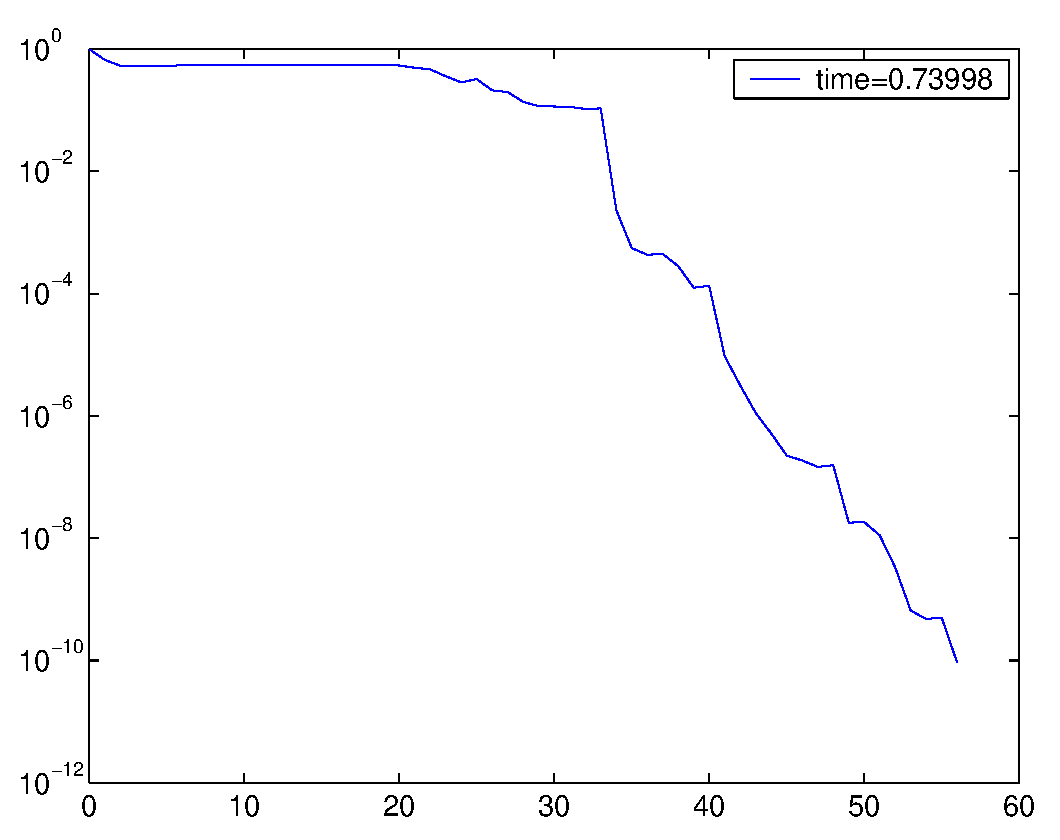
\includegraphics[scale=0.35]{eps/mp3qmrN20e50.eps}\hfill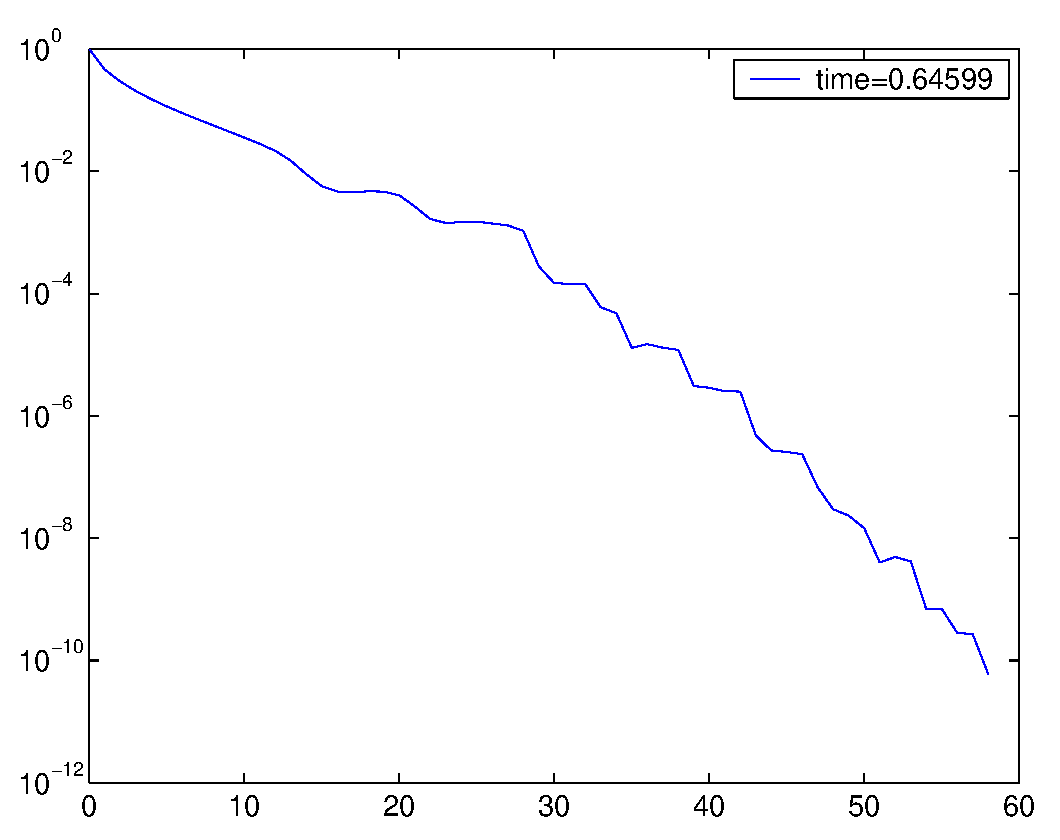
\includegraphics[scale=0.35]{eps/mp3qmrN20e1.eps}
\caption{Konvergenzgeschichte f"ur QMR. Links:$N=20, \epsilon = 50$, rechts $N=20, \epsilon = 1$}
\end{figure}

